% -*- coding: UTF-8 -*-
% vim: autoindent expandtab tabstop=4 sw=4 sts=4 filetype=tex
% chktex-file 27 - disable warning about missing include files

\section{Darstellung von impliziten Oberflächen}
\label{sec:description_implicit_surfaces}

Wie~\cite{hart_sphere_1994}[S. 1] angibt, existieren verschiedene Möglichkeiten
zur Darstellung (zum Rendering) von impliziten Oberflächen. So wandeln
indirekte Methoden implizite Oberflächen in Polygonmodelle um, was die Nuztung
bestehender Techniken und Hardware zur Darstellung von polygonalen Modellen
erlaubt. Obwohl die Umwandlung der impliziten Oberflächen mit gängigen Systemen
zur Darstellung problemlos dargestellt werden kann, ist die Umwandlung jedoch nicht
in jedem Fall gegeben und kann zu nicht zusammenhängenden Flächen oder einer
Verminderung des Detailgrades führen.\\
\\
Eine andere Methode zur Darstellung von impliziten Oberflächen ist das
unter~\ref{sec:ray_tracing} vorgestellte Ray Tracing Verfahren.

Ein (Licht-) Strahl wird dabei parametrisch als

\begin{gather}\label{eq:ray_param}
    r(t) = r_{0} + t \cdot r_{d}
\end{gather}

beschrieben. Der Strahl startet dabei bei Punkt $r_{0}$ in Richtung des
Einheitsvektors $r_{d}$, wobei $t$ die zurückgelegte Distanz des Strahles ist.
Dabei ist $r(t)$ der Punkt im Raum, welchen der Strahl nach dem Zurücklegen der
Distanz $t$ --- ausgehend von seinem Ursprung $r_{0}$ --- erreicht.\\
\\
Um nun die Schnittpunkte eines Strahles mit einer impliziten Oberfläche zu finden, wird die Gleichung des Lichtstrahles $r$ (\ref{eq:ray_param}) in die Funktion einer impliziten Oberfläche $f$ (\ref{eq:surface_implicit}) eingesetzt. Wobei $r : \mathbb{R} \to \mathbb{R}^{3}$ und $f : \mathbb{R}^{3} \to \mathbb{R}$. Dies ergibt die zusammengesetzte Funktion $F = f \circ r$ wobei $F : \mathbb{R} \to \mathbb{R}$.\\
\\
Die Lösungen dieser Gleichung sind alle Distanzen $t$, welche ein gegebener Strahl zurücklegt und welche die folgende Bedingung erfüllen:

\begin{gather}\label{eq:ray_param_cond}
    F(t) = f \circ r = f(r(t)) = 0
\end{gather}

Um die Gleichung~\ref{eq:ray_param_cond} zu lösen, können numerische Verfahren
zur Nullstellensuche angewendet werden, wobei die Verfahren vom Typ der
Funktion $F(t)$ abhängig sind. Bei polynomialen Funktionen bis zum vierten Grad
existieren analytische Lösungen, für eine beliebige Funktion muss jedoch ein
generisches, robustes Verfahren zur Nullstellensuche verwendet werden. Dies
bedingt jedoch meist, dass mehr Informationen über die Funktion zur Verfügung
stehen, was beispielsweise durch Ableiten dieser gelöst werden kann.\\
\\
Die erwähnten Verfahren zur Nullstellensuche haben jedoch häufig den Nachteil,
dass sie mehrere Schnittpunkte eines Strahles mit einer impliziten Oberfläche
liefern. Um diese Problematik zu umgehen, wird nur der kleinste Wert von $t$
berücksichtigt. Die Ray Marching und Sphere Tracing Algorithmen gehen hier
sogar noch einen Schritt weiter, in dem sie nur die kleinste positive
Nullstelle der Gleichung~\ref{eq:ray_param_cond} betrachten.

\subsection{Ray Marching}
\label{subsec:ray_marching}

~\cite{perlin_hypertexture_1989} schlagen eine Abtastung des Strahles mit fixen
Abständen $\Delta \mu$ vor:

\begin{gather}
    x = x_{\mu_{0}} + k \cdot \Delta x_{\mu}
\end{gather}

wobei $k = 0,1,2,\dots$ und $\mu_{0} + k \Delta \mu \leq \mu_{1}$.\\
\\
Auf die parametrische Darstellung eines (Licht-) Strahles,
Gleichung~\ref{eq:ray_param_cond}, angwendet:

\begin{gather}
    r(k) = r_{0} + \Delta t \cdot k \cdot r_{d}
\end{gather}

wobei $\Delta t$ die Grösse der Abstände und $k = 0,1,2,\dots$ die Nummer der
Schritte darstellt. Wie~\cite{hart_ray_1989} schreiben, bildet das Abtasten des
(Licht-) Strahles mit fixen Abständen die Basis für gewisse Verfahren des
volumetrischen Renderings.\\
\\
Ein möglicher Algorithmus, wie solch ein Verfahren umgesetzt werden kann,
findet sich in~\ref{fig:ray_marching}.

\begin{lstlisting}[language=Python,caption={Eine abstrakte Umsetzung des Ray
        Marchings\protect\footnotemark.},label={fig:ray_marching},captionpos=b,emph={ray_march}]
def ray_march():
    step         = 0
    intersection = 0
    max_steps    = 10

    while step < max_steps:
        intersection = test_intersection(k)

        if intersection <= 0:
            # An intersection has happened
            #   intersection <  0: ray is inside surface
            #   intersection == 0: ray is excatly on surface
            return ray_travel_distance(step)

        step = step + 1

    # When we reach this step, after max_steps, no intersection
    # has happened, so distance is 0
    return 0
\end{lstlisting}
\footnotetext{Algorithmus in Pseudocode
    gemäss~\cite{perlin_hypertexture_1989}[S. 259, Abschnitt 3.1]}

Dabei ist jedoch zu beachten, dass der Abstand zur Abtastung eines Strahles
$\Delta t$ so gering als möglich sein sollte um eine Punktemeng bzw.\ ein
Objekt --- definiert durch implizite Oberflächen --- $A$ möglichst gut
abschätzen zu können. Ist der gewählte Abstand zu gross gewählt, so findet ggf.
eine Abtastung weit im Inneren des Objektes statt und somit geht Präzision
verloren.  Es ist auch möglich dass der erste eigentliche Punkt gar nicht
abgetastet wird und erst der zweite abgetastete Punkt das Objekt ``erkennt''.

\begin{figure}[H]
    \caption{Illustration des Ray Marching Verfahrens und dessen
    Problemen.\protect\footnotemark}\label{fig:ray_marching_problems}
    \centering
    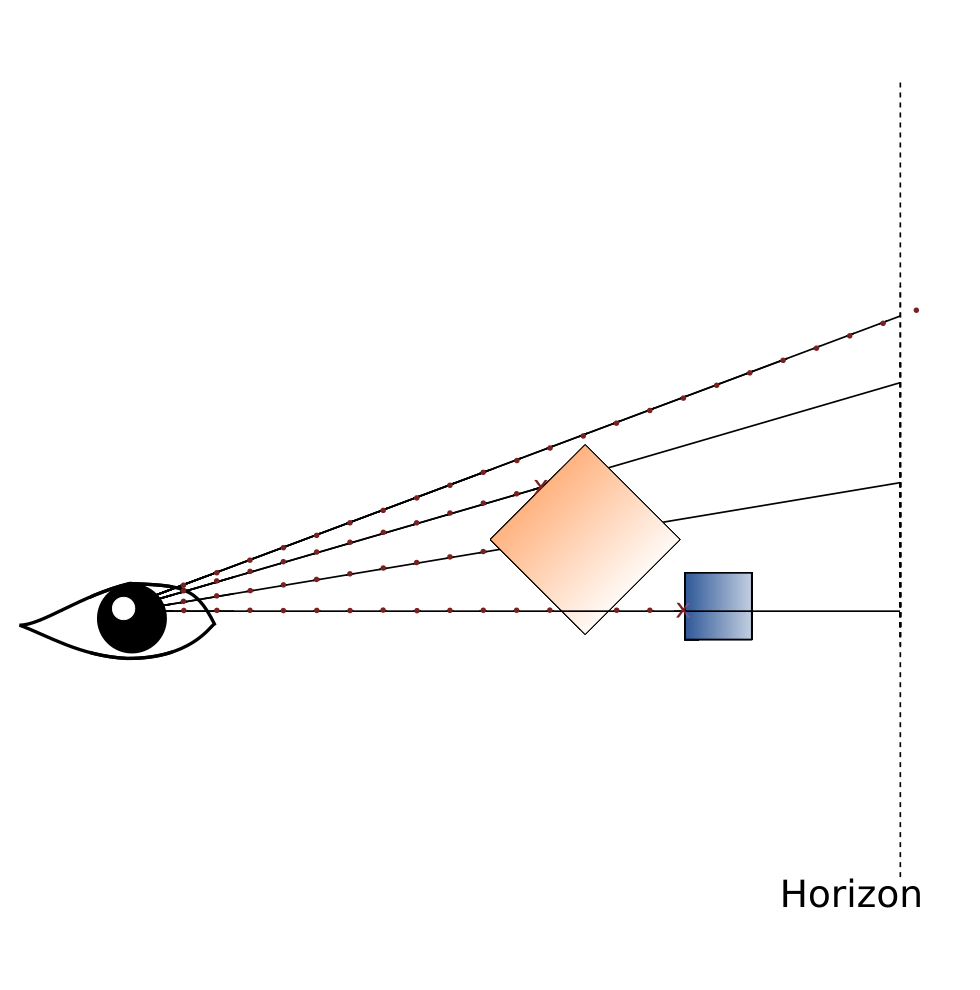
\includegraphics[width=0.5\textwidth]{img/ray_marching_problems.png}
\end{figure}
\footnotetext{Eigene Darstellung mittels Geogebra.}

Die Abbildung~\ref{fig:ray_marching_problems} veranschaulicht diese
Problematiken. Zu sehen sind vier Primärstrahlen, \textit{e},
\textit{f}, \textit{g} und \textit{h},  sowie zwei Objekte,
\textit{poly1} und \textit{poly2}.

Bei den Strahlen \textit{e} und \textit{g} handelt es sich um
``normale'' Fälle: Der Strahl \textit{e} geht komplett an den Objekten
vorbei, das Ray Marching wird also nach erreichen der maximalen Distanz
\textit{d\textsubscript{max}} abgebrochen, der Strahl \textit{g} trifft
das Objekt \textit{poly1} nach 6 Schritten.

Bei den Strahlen \textit{f} und \textit{h} handelt es sich um
Spezialfälle: Der Strahl \textit{f} trifft das Objekt \textit{poly1}
nicht, obwohl der Strahl durch das Objekt hindurch geht. Dies geschieht
aufgrund der gewählten Distanz zum Abtasten der Strahlen ($\Delta t$).
Der Strahl \textit{h} trifft das Objekt \textit{poly2}, obwohl er
eigentlich das Objekt \textit{poly1} treffen müsste. Das getroffene
Objekt \textit{poly2} dürfte so gar nicht zu sehen sein. Dieser Fehler
tritt wiederum aufgrund der gewählten Distanz zur Abtastung der Strahlen
($\Delta t$) auf.

\cite{hart_sphere_1994} weist darauf hin, dass Ray Marching durch den möglichst
geringen Abstand zwischen den Abtastungen entsprechend langsam und paralleles
Abtasten praktisch unumgänglich ist. In der von~\cite{hart_sphere_1994}
vorgestellten Technik des Sphere Tracings ist der Abstand zwischen den
Abtastungen nicht konstant sondern variiert in Abhängigkeit der Geometrie.

\subsection{Sphere Tracing}
\label{subsec:sphere_tracing}

Das von~\cite{hart_sphere_1994} vorgestellte Sphere Tracing Verfahren ist ein
Ray Tracing (\ref{sec:ray_tracing}) Verfahren für implizite Oberflächen. Es
handelt sich nach wie vor um Ray Marching (\ref{subsec:ray_marching}), die
Distanz der Schritte zum Abtastens  eines (Licht-) Strahles wird jedoch
aufgrund einer Distanzfunktion (\ref{ssubsec:distance_functions}) bestimmt.\\
\\
\cite{hart_sphere_1994} verweist auf den Term \textit{``unbounding volumes''},
welcher in~\cite{hart_ray_1989} eingeführt wurde. ``Unbounding volumes'' (zu
Deutsch etwa ``negativer Hüllkörper'') wird genutzt um Sphere Tracing zu
beschreiben und darzustellen. Der Term steht im Gegensatz zu dem gängigen
Konzept des Hüllkörpers (``bounding volumes'') --- ein Volumen, welches einen
Körper umschliesst. Ein ``negativer Hüllkörper'' (``unbounding volume'')
umschliesst also eine Fläche im Raum, welche den Körper \textit{nicht}
beinhaltet.\\
\\
Man möchte für einen abzutastenden Punkt im Raum ein Volumen finden, wessen
Zentrum im abzutastenden Punkt liegt. Ist der Abstand des Punktes zum nähesten
Punkt der Oberfläche eines Objektes bekannt, kann dieser Abstand als Radius
einer Kugel angenommen werden. Diese Kugel dient als negativer Hüllkörper
(``unbounding Volume'') und ist \textit{garantiert nicht} Teil des Objektes und
schneidet dieses auch nicht (ist also nicht $\overset{\circ}{\bm{A}}$) --- nur
der äusserste Punkt des Abstandes (also des Radius der Kugel) liegt genau auf
der Oberfläche des Objektes ($\partial \bm{A}$). Der Radius solch einer Kugel
wird durch Evaluation der Distanzfunktion eines abzutastenden Punktes im Raum
bestimmt.\\
\\
Gemäss~\cite{hart_sphere_1994} kommt daher auch der Name Sphere Tracing: Die
Schnittpunkte eines (Licht-) Strahles werden durch eine Folge von negativen
Hüllkörpern (``unbounding volumes'') --- bzw.\ in diesem Fall Kugeln
(``unbounding spheres'') --- beschrieben.\\
\\
Da~\cite{hart_ray_1989} die Darstellung von Fraktale im dreidimensionalen Raum
beschreibt, wird dort von einer Abschätzung der Distanz gesprochen. Dies ist
dadurch bedingt, dass die Distanz für Fraktale nicht effizient berechnet werden
kann. Betrachtet man jedoch die Darstellung von  ``regulären'' Objekten, wie zum
Beispiel eine Kugel, kann der zur Oberfläche am nähesten gelegene Punkt von
einem beliebigen Punkt derselben Domäne exakt berechnet werden. Dies ist durch
die implizite Gleichung~\ref{eq:surface_implicit_sphere} gegeben.\\
\\
Gemäss~\cite{hart_ray_1989} verläuft die Strahlenverfolgung bei dem Sphere
Tracing Verfahren wie folgt. Ein Strahl wird vom Betrachter (Auge bzw.
Lochkamera) durch die Bildebene zu einem Objekt geschossen. Dabei wird beim
initialen Augangspunkt der Radius eines negativen Hüllkörpers in Form einer
Kugel --- so wie oben beschrieben --- berechnet. Dies ist die Distanz, welcher
der Strahl in einem ersten Schritt effektiv zurücklegen wird. Bei jedem
Schnittpunkt der Kugel mit dem Strahl wird dasselbe Verfahren wiederholt. Dies
geschieht so lange, bis schliesslich der Strahl durch einen Schnittpunkt mit
einem Radius auf die Oberfläche des Objektes trifft. Ein weiteres
Abbruchkriterium ist eine definierte maximale Distanz eines Strahles. Ist diese
erreicht und der Strahl erreicht die Oberfläche des Objektes nicht --- weil der
Strahl das Objekt nicht schneidet oder das Objekt zu weit weg ist ---, wird
abgebrochen. Somit ist auch ersichtlich, dass Sphere Tracing nicht die
unter~\ref{subsec:ray_marching} genannten Problematiken aufweist.


\begin{figure}[H]
    \caption{Illustration des Sphere Tracing Verfahrens.\protect\footnotemark}\label{fig:sphere_tracing_1}
    \centering
    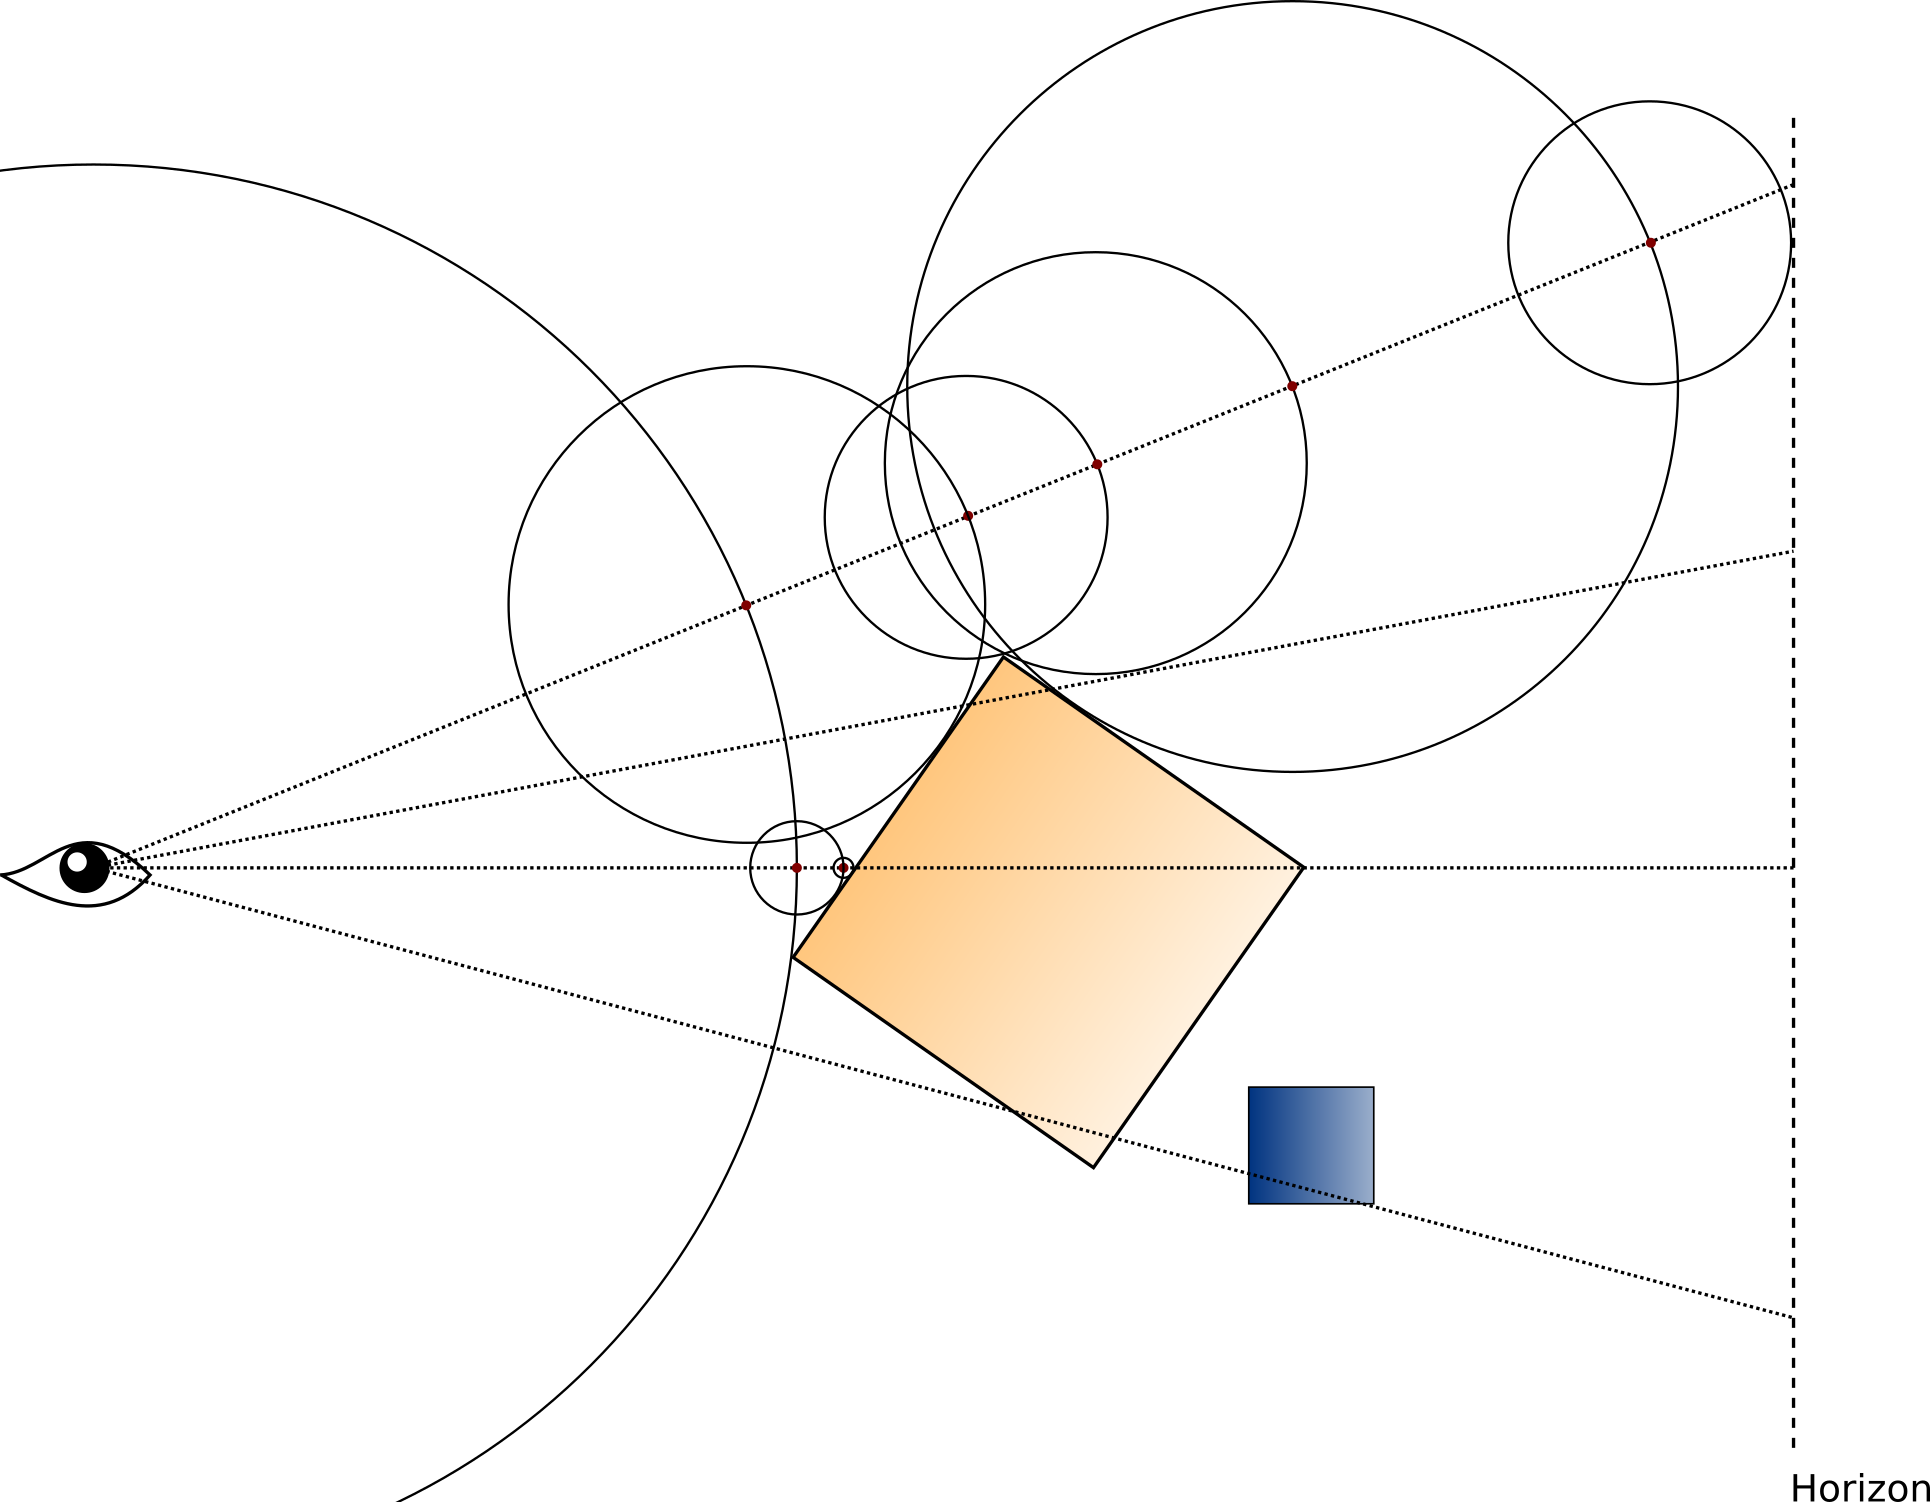
\includegraphics[width=1.0\textwidth]{img/sphere_tracing_principle.png}
\end{figure}
\footnotetext{Eigene Darstellung mittels Inkscape.}
\begin{figure}[H]
    \caption{Illustration des Sphere Tracing Verfahrens, Nahaufnahme.\protect\footnotemark}\label{fig:sphere_tracing_2}
    \centering
    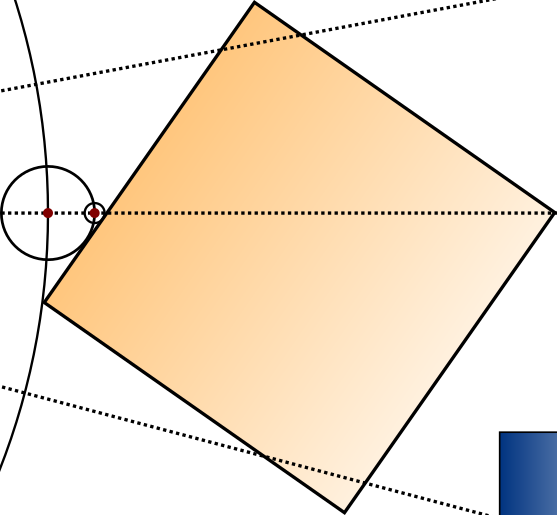
\includegraphics[width=0.5\textwidth]{img/sphere_tracing_principle_1.png}
\end{figure}
\footnotetext{Eigene Darstellung mittels Inkscape.}
\begin{table}[H]
    \centering
    \caption{INSERT CAPTION HERE\protect\footnotemark}\label{table:sphere_tracing_3}
    \begin{tabular}{p{0.3\textwidth}p{0.3\textwidth}p{0.3\textwidth}}
        \toprule
            \textbf{kShadow: \textit{8.0}} &
            \textbf{kShadow: \textit{16.0}}   &
            \textbf{kShadow: \textit{32.0}}   \\
        \cmidrule(r){1-1}\cmidrule(lr){2-2}\cmidrule(l){3-3}
            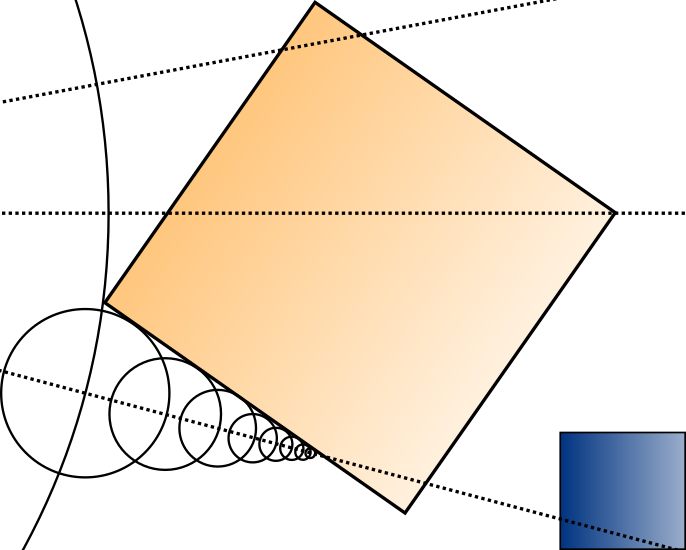
\includegraphics[width=0.3\textwidth]{img/sphere_tracing_principle_3_0.png} \newline &
            
\includegraphics[width=0.3\textwidth]{img/sphere_tracing_principle_3_1.png} \newline &
            \includegraphics[width=0.3\textwidth]{img/sphere_tracing_principle_3_2.png} \newline \\
        \bottomrule
    \end{tabular}
\end{table}
\footnotetext{Eigene Darstellung mittels Inkscape.}

Ausgehend von der parametrischen Beschreibung eines (Licht-) Strahles
(Gleichung~\ref{eq:ray_param}), beschreibt~\cite{hart_sphere_1994} die Richtung
$r_{d}$ eines Strahles als Einheitsvektor:

\begin{gather}
    r_{d} = \frac{p_{x, y} - r_{0}}{|p_{x, y} - r_{0}|}
\end{gather}

wobei $r_{0}$ der Ursprung eines Strahles und $p_{x, y}$ ein Punkt der Bildebene ist.\\
\\
Um nun den Schnittpunkt eines Strahles $r_{d}$ mit der Oberfläche eines
Objektes zu finden, muss die Gleichung $F(t)$ (\ref{eq:ray_param_cond}) gelöst
werden. Dabei ist --- wie oben definiert --- die Funktion $f(x)$ nun eine
Distanzfunktion wie die geometrische Distanzfunktion zur Beschreibung einer
Kugel (Gleichung~\ref{eq:surface_immplicit_geometric}).\\
\\
Evaluiert man nun die Gleichung $F(t)$ unter Anwendung der eben beschriebenen
Strahlenverfolgung, findet man so die erste positive Nullstelle der Gleichung
$F(t)$. Diese Nullstelle ist die Grenze der Folge von negativen Hüllkörpern
(``unbounding spheres''), welche durch die rekursive Gleichung:

\begin{gather}
    t_{i+1} = t_{i} + F(t_{i})
\end{gather}

definiert ist. Der Ursprungspunkt ist dabei als $t_{0}$ definiert. Diese Folge
konvergiert genau dann --- und nur dann --, wenn der Strahl auf die implizite
Oberfläche eines Objkektes trifft. Diese Folge bildet den Kern des Algorithmus
zur Darstellung von geometrisch definierten, impliziten Oberflächen.

\begin{lstlisting}[language=Python,caption={Eine abstrakte Umsetzung des Sphere
        Tracings\protect\footnotemark.},label={alg:sphere_tracing},captionpos=b,emph={sphere_trace}]
def sphere_trace():
    ray_distance          = 0
    estimated_distance    = 0
    max_distance          = 9001
    convergence_precision = 0.000001

    while ray_distance < max_distance:
        # sd_sphere is a signed distance function defining the implicit surface
        # cast_ray defines the ray equation given the current travelled /
        # marched distance of the ray
        estimated_distance = sd_sphere(cast_ray(ray_distance))

        if estimated_distance < convergence_precision:
            # the estimated distance is already smaller than the desired
            # precision of the convergence, so return the distance the ray has
            # travelled as we have an intersection
            return ray_distance

        ray_distance = ray_distance + estimated_distance

    # When we reach this point, there was no intersection between the ray and a
    # implicit surface, so simply return 0
    return 0
\end{lstlisting}
\footnotetext{Algorithmus in Pseudocode gemäss~\cite{hart_sphere_1994}[S. 531,
    Fig. 1]}

\subsection{Operationen für implizite Oberflächen}
\label{subsec:implicit_surfaces_ops}

Um mit impliziten Oberflächen nicht nur einfache Objekte, wie zum Beispiel eine
Kugel darzustellen, möchte man diese auch transformieren können.

Wie~\cite{hart_sphere_1994}[S. 543] beschreibt, werden implizite Oberflächen
durch die Invertierung des Raumes, in welchem sich die Oberfläche befindet,
transformiert. Der Raum, in dem sich eine implizite Oberfläche befindet, ist
die Domäne der impliziten Funktion der Oberfläche.

Sei $T(\bm{x})$ eine Transformation und $f(\bm{x})$ eine Distanzfunktion,
welche eine implizite Oberfläche definiert. Somit ist die transfomierte
implizite Oberfläche:

\begin{gather}
    f(T^{-1}(\bm{x})) = 0
\end{gather}

Bei Transformationen handelt es sich um vorzeichenabhängige Distanzfunktion
(signed distance functions).

Es werden dabei folgende Arten von Transformationen unterschieden:
\begin{itemize}
    \item Distanzoperationen, wie zum Beispiel Vereinigung, Subtraktion oder Intersektion
    \item Domänenoperationen, wie zum Beispiel Wiederholung, Rotation, Translation und Skalierung
    \item Distanzdeformationen, wie zum Beispiel Versatz (displacement) und Vermengung/Vermischung (blend)
    \item Domänendeformationen, wie zum Beispiel ``Verderung'' (twist) und Biegung (bend)
\end{itemize}

\subsubsection{Isometrien}
\label{ssubsec:implicit_surfaces_ops_isometries}

Nicht alle Transformationen erhalten dabei die Distanz, welche die
Distanzfunktion der transformieren Oberfläche zurückgeben würde. In solch einem
Falle ist die zurückgegebene Distanz nicht die Distanz eines beliebigen Punktes
im Raum zu dem ihm nähesten Punkt einer impliziten Oberfläche.

Transformationen, welche hingegen distanzerhaltend sind,
bezeichnet~\cite{hart_sphere_1994} als~\textit{Isometrien}. Dazu zählen
Rotationen, Translationen aber auch Reflektionen.

Ist $\bm{I}$ eine Isometrie, dann benötigt die zurückgegebene Distanz der
Distanzfunktion $f(\bm{x})$ \textit{keine Anpassung}.

\begin{gather}
    d(\bm{x}, \bm{I} \circ f^{-1}(0)) = d(\bm{I}^{-1}(\bm{x}), f^{-1}(0))
\end{gather}

Wobei $\bm{I}$ eine Isometrie und $f^{-1}(0)$ eine implizite Oberfläche ist.

\subsubsection{Uniforme Skalierung}
\label{ssubsec:implicit_surfaces_ops_scaling}

Eine Skalierung ist \textit{nicht} distanzerhaltend, daher \textit{erhält} sie die Distanz, welche die
Distanzfunktion der skalierten Oberfläche zurückgeben würde, \textit{nicht}.
Somit muss die zurückgegebene Distanz entsprechend angepasst werden.

\cite{hart_sphere_1994} gibt die uniforme Skalierung als Transformation $\bm{S(x)}$  der Form:

\begin{gather}
    \bm{S(x)} = s \cdot \bm{x}
\end{gather}

an, wobei $s$ der Skalierungsfaktor ist. Die Invertierung der Skalierung ist gegeben als:

\begin{gather}
    \bm{S^{-1}(x)} = {1 \over s} \cdot \bm{x}
\end{gather}

Somit ist die Distanz zu der skalierten impliziten Oberfläche:

\begin{gather}
    d(\bm{x}, \bm{S}(f^{-1}(0))) = s \cdot d(\bm{S}^{-1}(\bm{x}), f^{-1}(0))
\end{gather}

Dabei wird die von der Distanzfunktion der skalierten impliziten Oberfläche
zurückgegebene Distanz mit dem Skalierungsfaktor $s$ multipliziert, was die
eigentliche Distanzinformation erhält und die Skalierung somit isometrisch
macht.

\subsubsection{``Verdrehung'' (Twist)}
\label{ssubsec:implicit_surfaces_ops_twist}

Gemäss~\cite{hart_sphere_1994}[S. 543] werden bei der ``Verdrehung'' einer
impliziten Oberfläche zwei Achsen (z.B. $x$ und $y$) anhand einer linearen Funktion $a(\cdot)$ in
Abhängigkeit der dritten Achse (z.B. $z$) rotiert:

\begin{gather}
    twist(\bm{x}) = \begin{pmatrix} 
        x \cdot \cos{a(z)} - y \cdot \sin{a(z)},\\
        x \cdot \sin{a(z)} + y \cdot \cos{a(z)},\\
        z
    \end{pmatrix}
\end{gather}

\subsubsection{Vereinigung}
\label{ssubsec:implicit_surfaces_ops_union}

Die Vereinigung zweier impliziter Oberflächen $A$ und $B$ wird
von~\cite{hart_sphere_1994} als minimale Distanz der jeweiligen
vorzeichenabhängigen  Distanzfunktion $f_{A}$ respektive $f_{B}$ definiert:

\begin{gather}
    d(\bm{x}, A \cup B) = \min(f_{A}(\bm{x}), f_{B}(\bm{x}))
\end{gather}

wobei $\bm{x}$ den abzutastenden Punkt im Raum darstellt.

Wie~\ref{hart_sphere_1994} schreibt, ist die Distanz zu einer Liste von
impliziten Oberflächen die kleinste Distanz der jeweiligen Distanzfunktion.
Somit erlaubt es die Vereinigung --- neben der Kombination von Objekten ---
mehrere implizite Oberflächen zu kombinieren, ohne dass diese miteinander in
Kontakt stehen müssen. So kann beispielsweise eine komplexe Szene modelliert
werden.

\subsubsection{Subtraktion}
\label{ssubsec:implicit_surfaces_ops_subtraction}

Um die Operation der Subtraktion zu definieren, wird die Distanz zum Komplement
eines Objektes $\bm{A}$ verwendet. Dabei wird die Eigenschaft der
Vorzeichenabhängigkeit von vorzeichenabhängigen Distanzfunktionen genutzt:

\begin{gather}
    d(\bm{x}, \mathbb{R}^{3} \setminus A) = -f_{A}(\bm{x})
\end{gather}

Somit kann die Subtraktion zweier impliziter Oberflächen $A$ und $B$
gemäss~\cite{hart_sphere_1994} als Intersektion eines Objektes $A$ mit der
Subtraktion des Raumes bzw.\ der Domäne mit einem Objekt $B$ angesehen werden,
daher folgt:

\begin{align}
    d(\bm{x}, A - B) &= A \cap (\mathbb{R}^{3} \setminus B) \\
                     &\geq \max(f_{A}(\bm{x}), -f_{B}(\bm{x}))
\end{align}

wobei $\bm{x}$ den abzutastenden Punkt im Raum darstellt.

\subsubsection{Intersektion}
\label{ssubsec:implicit_surfaces_ops_intersection}

Die Intersektion zweier impliziter Oberflächen $A$ und $B$ wird
von~\cite{hart_sphere_1994} als minimale Distanz der jeweiligen
vorzeichenabhängigen  Distanzfunktion $f_{A}$ respektive $f_{B}$ definiert:

\begin{gather}
    d(\bm{x}, A \cap B) \geq \max(f_{A}(\bm{x}), f_{B}(\bm{x}))
\end{gather}

wobei $\bm{x}$ den abzutastenden Punkt im Raum darstellt.

\subsection{Primitive}
\label{subsec:implicit_surfaces_primitives}

\cite{hart_sphere_1994} führt in seinem Paper einige (geometrische) Primitve
auf, welche nachfolgende erläutert werden.

\subsubsection{Ebene}
\label{ssubsec:implicit_surfaces_primitives_plane}

Die vorzeichenbehaftete Distanz zu einer Ebene $P$ mit einer Einheitsnormalen $\bm{n}$, welche sich mit dem Punkt $\bm{n} \cdot r$ schneidet ist wie folgt:

\begin{gather}
    d(\bm{x}, P) = \bm{x} \cdot \bm{n} - r
\end{gather}

wobei $r$ die relative Positionierung der Ebene --- unter Einbezug der Normalen der Ebene im Verhältnis zur Eintheistnormalen $\bm{n}$ --- im Raum darstellt.

\subsubsection{Kugel}
\label{ssubsec:implicit_surfaces_primitives_sphere}

Eine Kugel ist als eine Menge von Punkten (Locus) in fixem Abstand eines gegebenen Punktes. Die vorzeichenbehaftete Distanz zu einer Kugel $S$, ausgehend vom Ursprung, ist wie folgt:

\begin{gather}
    d(\bm{x}, S) = \|\bm{x}\| - r
\end{gather}

wobei $r$ den Radius der Kugel darstellt.

\subsubsection{Zylinder}
\label{ssubsec:implicit_surfaces_primitives_cylinder}

Die Distanz zu einem um die Z-Achse zentrierten Zylinder mit Einheitsradius wird durch Projektion auf die XY-Ebene und Messung der Distanz zum Einheitskreis berechnet:

\begin{gather}
    d(\bm{x}, Cyl) = \|(x, y)\| - r
\end{gather}

wobei $r$ den Radius des Zylinders darstellt, $\bm{x}$ stellt dabei $(x,y,z)$ dar.

\subsubsection{Kegel}
\label{ssubsec:implicit_surfaces_primitives_cone}

Die Distanz zu einem Kegel, welcher am Ursprsung zentriert und entlang der Z-Achse orientiert ist, wird wie folgt berechnet:

\begin{gather}
    d(\bm{x}, Cone) = \|(x, y)\| \cdot \cos(\phi) - |z| \cdot \sin(\phi)
\end{gather}

wobei $\phi$ den Winkel zur Z-Achse darstellt.

\subsubsection{Torus}
\label{ssubsec:implicit_surfaces_primitives_torus}

Beim Torus handelt es sich um das Produkt zweier Kreise, sowie den Abstand der Kreise:

\begin{gather}
    d(\bm{x}, T) = \|(\|(x, y)\| - R, z)\| - r
\end{gather}

wobei $R$ den Aussenradius und $r$ den Innenradius des Torus darstellt. Der Torus ist am Ursprung zentriert und dreht sich um die Z-Achse.
